\documentclass[12pt, psamsfonts]{amsart}

%-------Packages---------
\usepackage{amssymb,amsfonts}
\usepackage{fullpage}
\usepackage{tikz-cd}
\usepackage{todonotes}
\usepackage{physics}
\usepackage[all,arc]{xy}
\usepackage{enumerate}
\usepackage{enumitem}
\usepackage{mathrsfs}
\usepackage{theoremref}
\usepackage{graphicx}
\usepackage[bookmarks]{hyperref}

%--------Theorem Environments--------
%theoremstyle{plain} --- default
\newtheorem{thm}{Theorem}[section]
\newtheorem{cor}[thm]{Corollary}
\newtheorem{prop}[thm]{Proposition}
\newtheorem{lem}[thm]{Lemma}
\newtheorem{conj}[thm]{Conjecture}
\newtheorem{quest}[thm]{Question}

\theoremstyle{definition}
\newtheorem{defn}[thm]{Definition}
\newtheorem{defns}[thm]{Definitions}
\newtheorem{con}[thm]{Construction}
\newtheorem{exmp}[thm]{Example}
\newtheorem{exmps}[thm]{Examples}
\newtheorem{notn}[thm]{Notation}
\newtheorem{notns}[thm]{Notations}
\newtheorem{addm}[thm]{Addendum}
\newtheorem*{exer}{Exercise}

\theoremstyle{remark}
\newtheorem{rem}[thm]{Remark}
\newtheorem{rems}[thm]{Remarks}
\newtheorem{warn}[thm]{Warning}
\newtheorem{sch}[thm]{Scholium}

\DeclareMathOperator{\Hom}{Hom}
\DeclareMathOperator{\Id}{Id}

\makeatletter
\let\c@equation\c@thm
\makeatother
\numberwithin{equation}{section}

\bibliographystyle{plain}

\begin{document}

\title{Math 611 Homework (Due 10/16)}
\author{Hidenori Shinohara}
\maketitle

\begin{exer}{(Problem 16)}
  Given maps $X \rightarrow Y \rightarrow Z$ such that both $Y \rightarrow Z$ and the composition $X \rightarrow Z$ are covering spaces, show that $X \rightarrow Y$ is a covering space if $Z$ is locally path-connected, and show that this covering space is normal if $X \rightarrow Z$ is a normal covering space.
\end{exer}

\begin{proof}
  Let $p: X \rightarrow Y, q: Y \rightarrow Z$ be given such that $q$ and $q \circ p$ are both covering maps.
  Let $y_0 \in Y$ be given.
  It suffices to show that there exists a neighborhood of $y_0$ that is evenly covered by $p$.
  (Hatcher does not require a covering map be surjective.)

  Let $z_0 = q(y_0)$.
  Let $U_{z_0}$ be a locally path-connected neighborhood of $z_0$ contained in the intersection of the following two neighborhoods:
  \begin{itemize}
    \item
      A neighborhood of $z_0$ that is evenly covered by $q$.
    \item
      A neighborhood of $z_0$ that is evenly covered by $q \circ p$.
  \end{itemize}

  Those two neighborhoods of $z_0$ must exist because $q$ and $q \circ p$ are covering maps.
  Since $Z$ is locally path-connected, any neighborhood of $z_0$ contains a path-connected neighborhood of $z_0$.
  Therefore, such $U_{z_0}$ must exist.
  Moreover, any neighborhood contained in an evenly covered neighborhood is evenly covered.
  Therefore, $U_{z_0}$ is a path-connected neighborhood of $z_0$ that is evenly covered by both $q$ and $q \circ p$.

  Since $U_{z_0}$ is evenly covered by $q$ and $q \circ p$,
  \begin{itemize}
    \item
      Let $\coprod_{\alpha} U_{x_{\alpha}} = (q \circ p)^{-1}(U_{z_0})$ where $q \circ p$ maps each $U_{x_{\alpha}}$ into $U_{z_0}$ homeomorphically.
    \item
      Let $\coprod_{\beta} U_{y_{\beta}} = q^{-1}(U_{z_0})$ where $q$ maps each $U_{y_{\beta}}$ into $U_{z_0}$ homeomorphically.
  \end{itemize}

  Since $z_0 = q(y_0)$ and $q$ is an covering map, there exists $U_{y_{\beta}}$ such that $y_0 \in U_{y_{\beta}}$.
  For simplicity, we will call it $U_{y_0}$.
  In other words, $U_{y_0}$ is a neighborhood of $y_0$ such that $q$ is a homeomorphism between $U_{y_0}$ and $U_{z_0}$.

  We claim that $U_{y_0}$ is a neighborhood of $y_0$ that is evenly covered by $p$ by showing that there exists a subset $I$ of the index set such that $p^{-1}(U_{y_0}) = \coprod_{\alpha \in I} U_{x_{\alpha}}$.


  We claim that for all $\alpha$, $U_{x_{\alpha}} \subset p^{-1}(U_{y_0})$ or $U_{x_{\alpha}} \cap p^{-1}(U_{y_0}) = \emptyset$.
  Let $\alpha$ be given.
  Suppose $U_{x_{\alpha}} \cap p^{-1}(U_{y_0}) \ne \emptyset$.
  Let $x \in U_{x_{\alpha}} \cap p^{-1}(U_{y_0})$.
  Let $x' \in U_{x_{\alpha}}$.
  We will show that $x' \in p^{-1}(U_{y_0})$.

  Since $U_{z_0}$ is path connected and $U_{x_{\alpha}}$ is homeomorphic to $U_{z_0}$, $U_{x_{\alpha}}$ is path connected.
  Let $\gamma$ be a path from $x$ to $x'$.
  In other words, $\gamma(0) = x$ and $\gamma(1) = x'$.
  Then $q \circ p \circ \gamma$ is a path in $U_{z_0}$.
  Let $z = (q \circ p \circ \gamma)(0), z' = (q \circ p \circ \gamma)(1)$.
  Then $q \circ p \circ \gamma$ is a path from $z$ to $z'$ in $U_{z_0}$.
  Since $U_{z_0}$ and $U_{y_0}$ are homeomorphic by $q$, there exists a unique point $y \in U_{y_0}$ such that $q(y) = z$.
  Since $q$ is a covering map, there exists a unique lift $\widetilde{q \circ p \circ \gamma}$ based at $y$.
  Let $y' = \widetilde{q \circ p \circ \gamma}(1)$.
  Then $y' \in U_{y_0}$ because the lift must entirely lie in $U_{y_0}$ because $q$ is a homeomorphism between $U_{y_0}$ and $U_{z_0}$.

  Consider the path $p \circ \gamma$ in $Y$.
  Since $(p \circ \gamma)(0) = p(x)$ and $x \in p^{-1}(U_{y_0})$, the initial point of $p \circ \gamma$ is in $U_{y_0}$.
  Moreover, $q(p(x)) = z$ and $y$ is the unique point in $U_{y_0}$ such that $q(y) = z$, $y = p(x)$.
  Since $q \circ (p \circ \gamma) = (q \circ p) \circ \gamma$, $p \circ \gamma$ is also a lift of $q \circ p \circ \gamma$ based at $y$.
  By the uniqueness of a lift, $\widetilde{q \circ p \circ \gamma} = p \circ \gamma$.
  Specifically, this implies that $p(x') = (p \circ \gamma)(1) = \widetilde{q \circ p \circ \gamma}(1) = y' \in U_{y_0}$.
  Since $p(x') \in U_{y_0}$, $x' \in p^{-1}(U_{y_0})$.

  Let $I = \{ \alpha \mid U_{x_{\alpha}} \subset p^{-1}(U_{y_0}) \}$.
  Then we have $\coprod_{\alpha \in I} U_{x_{\alpha}} \subset p^{-1}(U_{y_0})$.

  Since $p^{-1}(U_{y_0}) \subset p^{-1}(q^{-1}(U_{z_0})) = \coprod_{\alpha} U_{x_{\alpha}}$, every point in $p^{-1}(U_{y_0})$ is in $U_{x_{\alpha}}$ for some $\alpha$.
  $I$ includes all $\alpha$ such that $U_{x_{\alpha}}$ intersects with $p^{-1}(U_{y_0})$.
  Thus $p^{-1}(U_{y_0}) \subset \coprod_{\alpha \in I} U_{x_{\alpha}}$.

  Therefore, $\coprod_{\alpha \in I} U_{x_{\alpha}} = p^{-1}(U_{y_0})$.

  Finally, we will show that $p$ is a homeomorphism between $U_{x_{\alpha}}$ and $U_{y_0}$.
  Let $\alpha \in I$.
  We claim that $p(U_{x_{\alpha}}) = U_{y_0}$.
  \begin{itemize}
    \item
      $p(U_{x_{\alpha}}) \subset U_{y_0}$ because of how we defined $I$.
    \item
      Let $y \in U_{y_0}$.
      Since $U_{y_0}$ is path connected, there exists a path $\gamma$ from $y_0$ to $y$ in $U_{y_0}$.
      Then $q \circ \gamma$ is a path in $U_{z_0}$.
      Since $q \circ p$ maps $U_{x_{\alpha}}$ into $U_{z_0}$ homeomorphically, there exists a unique $x_0 \in U_{x_{\alpha}}$ such that $(q \circ p)(x_0) = z_0$.
      By the unique lifting property, there exists a unique lift $\widetilde{q \circ \gamma}$ of $q \circ \gamma$ based at $x_0$.
      Again, since $q \circ p$ maps $U_{x_{\alpha}}$ into $U_{z_0}$ homeomorphically, $\widetilde{q \circ \gamma}$ is in $U_{x_{\alpha}}$.

      Then $p \circ (\widetilde{q \circ \gamma})$ is a path in $U_{y_0}$.
      Since $q \circ (p \circ (\widetilde{q \circ \gamma})) = (q \circ p) \circ (\widetilde{q \circ \gamma}) = q \circ \gamma$ and $q$ is a homeomorphism between $U_{y_0}$ and $U_{z_0}$, $\gamma = p \circ (\widetilde{q \circ \gamma})$.
      Then $p(\widetilde{q \circ \gamma}(1)) = (p \circ (\widetilde{q \circ \gamma}))(1) = \gamma(1) = y$.
      Thus $y \in p(U_{x_{\alpha}})$.
  \end{itemize}

  We know that $(q \circ p) \mid_{U_{x_{\alpha}}}$ and $q \mid_{U_{y_0}}$ are homeomorphisms.
  \begin{align*}
    (q \mid_{U_{y_0}})^{-1} \circ (q \circ p) \mid_{U_{x_{\alpha}}}
      &= (q \mid_{U_{y_0}})^{-1} \circ q \mid_{p(U_{x_{\alpha}})} \circ p \mid_{U_{x_{\alpha}}} \\
      &= (q \mid_{U_{y_0}})^{-1} \circ q \mid_{U_{y_0}} \circ p \mid_{U_{x_{\alpha}}} \\
      &= p \mid_{U_{x_{\alpha}}}
  \end{align*}
  Thus $p \mid_{U_{x_{\alpha}}}$ is a homeomorphism between $U_{x_{\alpha}}$ and $U_{y_0}$.

  In conclusion, $U_{y_0}$ is a neighborhood of $y_0$ such that $p^{-1}(U_{y_0})$ is the disjoint union $\coprod_{\alpha \in I} U_{x_{\alpha}}$ such that $p$ is a homeomorphism between each $U_{x_{\alpha}}$ and $U_{y_0}$.
  Therefore, $p$ is a covering map.

  Suppose that $q \circ p$ is normal.
  By Proposition 1.39(a), it suffices to show that $p_*\pi_1(X)$ is a normal subgroup of $\pi_1(Y)$.
  Let $p_*([h]) \in \pi_1(X)$ and $[g] \in \pi_1(Y)$.
  By Proposition 1.39(a), $(q \circ p)_*(\pi_1(X)) = q_*(p_*(\pi_1(X)))$ is a normal subgroup of $\pi_1(Z)$.
  Therefore, $q_*([g] p_*([h]) [g]^{-1}) = q_*([g])q_*(p_*([h]))q_*([g])^{-1} = q_*(p_*([h']))$ for some $[h'] \in \pi_1(X)$.
  Since $q_*$ is injective by Proposition 1.31, $[g]p_*([h])[g]^{-1} = p_*([h]') \in p_*(\pi_1(X))$.
  Thus $p_*(\pi_1(X))$ is a normal subgroup of $\pi_1(Y)$.
\end{proof}

\begin{exer}{(Problem 18)}
  For a path-connected, locally path-connected, and semilocally simply-connected space $X$, call a path-connected covering space $X \rightarrow X$ abelian if it is normal and has abelian deck transformation group.
  Show that $X$ has an abelian covering space that is a covering space of every other abelian covering space of $X$, and that such a `universal' abelian covering space is unique up to isomorphism.
  Describe this covering space explicitly for $X = S^1 \vee S^1$ and $X = S^1 \vee S^1 \vee S^1$.
\end{exer}

\begin{proof}
  In this proof, we will invoke Proposition 1.39 without referring to it since it will be used so many times that the solution simply gets longer and less readable if we explicitly write it every time.
  We will consider the commutator subgroup $H = [\pi_1(X, x_0), \pi_1(X, x_0)]$ generated by $\{ [a, b] \mid a, b \in \pi_1(X, x_0) \}$ of $\pi_1(X, x_0)$.
  Since $H$ is a subgroup of $\pi_1(X, x_0)$ and $X$ is path-connected, locally path connected, and semilocally simply connected, there exists a path-connected covering space $p: (\tilde{X}, \tilde{x_0}) \rightarrow (X, x_0)$ such that $p_*(\pi_1(\tilde{X}, \tilde{x_0})) = H$ by Proposition 1.38.

  $G(\tilde{X})$ is isomorphic to the quotient $N(H) / H$.
  \begin{itemize}
    \item
      Since $H$ is the commutator subgroup, $H$ is a normal subgroup of $\pi_1(X, x_0)$.
      Thus $N(H) = \pi_1(X, x_0)$.
      Moreover, $\tilde{X}$ is normal because $H = p_*(\pi_1(\tilde{X}, \tilde{x_0}))$ is normal.
    \item
      Since $H$ is the commutator subgroup of $\pi_1(X, x_0) = N(H)$, $N(H) / H$ is abelian.
  \end{itemize}
  Therefore, $\tilde{X}$ is an abelian covering space of $X$.

  Let $p': \tilde{X}' \rightarrow X$ be an abelian covering space of $X$.
  Let $H' = p_*'\pi_1(\tilde{X}')$.
  Since $\tilde{X}'$ is a normal covering space, $G(\tilde{X}') = \pi_1(X) / H'$.
  Since $\pi_1(X) / H'$ is abelian, $H'$ must contain commutators $[a, b]$ for all $a, b \in \pi_1(X)$.
  Therefore,

  \begin{equation}
    \text{If $p': \tilde{X}' \rightarrow X$ is abelian , $[\pi_1(X), \pi_1(X)] \subset p_*'\pi_1(\tilde{X}')$.} \label{eq:abelian}
  \end{equation}

  We will refer to this result later.

  Thus $p_*(\pi_1(\tilde{X})) = [\pi_1(X), \pi_1(X)] \subset H' = p_*'(\pi_1(\tilde{X}'))$.
  By Proposition 1.33, there exists a lift $\tilde{p}$ such that $p = p' \circ \tilde{p}$.
  By Problem 16 from above, $p': \tilde{X} \rightarrow \tilde{X}'$ is a covering.
  Therefore, $\tilde{X}$ is a universal abelian covering.

  Let $q: Y \rightarrow Y$ be a universal abelian covering space of $X$.
  By \eqref{eq:abelian}, $q_*(\pi_1(Y))$ must contain all commutators.
  Since $q$ is a universal abelian covering space of $X$, there exists a covering map $q': Y \rightarrow \tilde{X}$ such that $p \circ q' = q$.
  Then $q'$ is a lift of $q$ with respect to $p$.
  By Proposition 1.33, this implies that $q_*(\pi_1(Y)) \subset p_*(\pi_1(\tilde{X})) = [\pi_1(X), \pi_1(X)]$.
  Thus $q_*(\pi_1(Y))$ is exactly the commutator subgroup.
  $p_*(\pi_1(\tilde{X})) = q_*(\pi_1(Y))$, so $\tilde{X}$ and $Y$ are isomorphic by Theorem 1.38.

  Therefore, $\tilde{X}$ is the `universal' abelian covering space that is unique up to isomorphism.

  Figure \ref{fig:problem18_s1_s1} shows the universal abelian covering spaces of $S^1 \vee S^1$ and $S^1 \vee S^1 \vee S61$.
  \begin{itemize}
    \item
      As shown in Figure \ref{fig:problem18_s1_s1}, we claim that the universal abelian covering space $\tilde{X}$ of $S^1 \vee S^1$ is $\{ (x, y) \in \mathbb{R}^2 \mid \{ x, y \} \cap \mathbb{Z} \ne \emptyset \}$.
      Each segment of length 1 between grid points corresponds to one of the circles as described in Figure \ref{fig:problem18_s1_s1}.
      $\tilde{X}$ is a normal covering because, for any grid point $(m, n)$, shifting $\tilde{X}$ by $m$ in the $x$ direction and $y$ in the $y$ direction gives a deck transformation mapping $(0, 0)$ to $(m, n)$.
      Since this is a bijective correspondence between translations of the space and deck transformations, $G(\tilde{X}) = \mathbb{Z}^2$.
      Since $\tilde{X}$ is normal, $G(\tilde{X}) = \pi_1(S^1 \vee S^1) / H$ where $H = p_*(\pi_1(\tilde{X}))$.
      Then $\ev{a, b} / H \cong \mathbb{Z}^2$, so $H$ must be the commutator subgroup of $\ev{a, b} = \pi_1(X)$.

      On the other hand, from the argument above, for a universal abelian covering space $q: Y \rightarrow S^1 \vee S^1$, $q_*(\pi_1(Y))$ is the commutator subgroup of $\pi_1(X)$.
      Thus $H = q_*(\pi_1(Y))$, so $\tilde{X}$ and $Y$ are isomorphism by Theorem 1.38.
    \item
       As shown in Figure \ref{fig:problem18_s1_s1}, we claim that the universal abelian covering space of $S^1 \vee S^1 \vee S^1$ is $\{ (x, y, z) \in \mathbb{R}^3 \mid \{ x, y, z \} \cap \mathbb{Z} \ne \emptyset \}$.
      Each segment of length 1 between grid points corresponds to one of the circles as described in Figure \ref{fig:problem18_s1_s1}.
      (In order to avoid drawing too many lines, I did not write the $xy$ plane for $z = -1, -2, \cdots$ in Figure \ref{fig:problem18_s1_s1}.)

      Using the exact same argument as above, we conclude that this is the universal abelian cover of $S^1 \vee S^1 \vee S^1$.
      (The deck transformation group is $\mathbb{Z}^3$.
      Since $\pi_1(S^1 \vee S^1 \vee S^1) = \ev{a, b, c}$, $p_*(\pi_1(\tilde{X}))$ is the commutator subgroup of $\ev{a, b, c}$.
      Thus $\tilde{X}$ is the universal abelian cover.)
  \end{itemize}

  \begin{figure}
    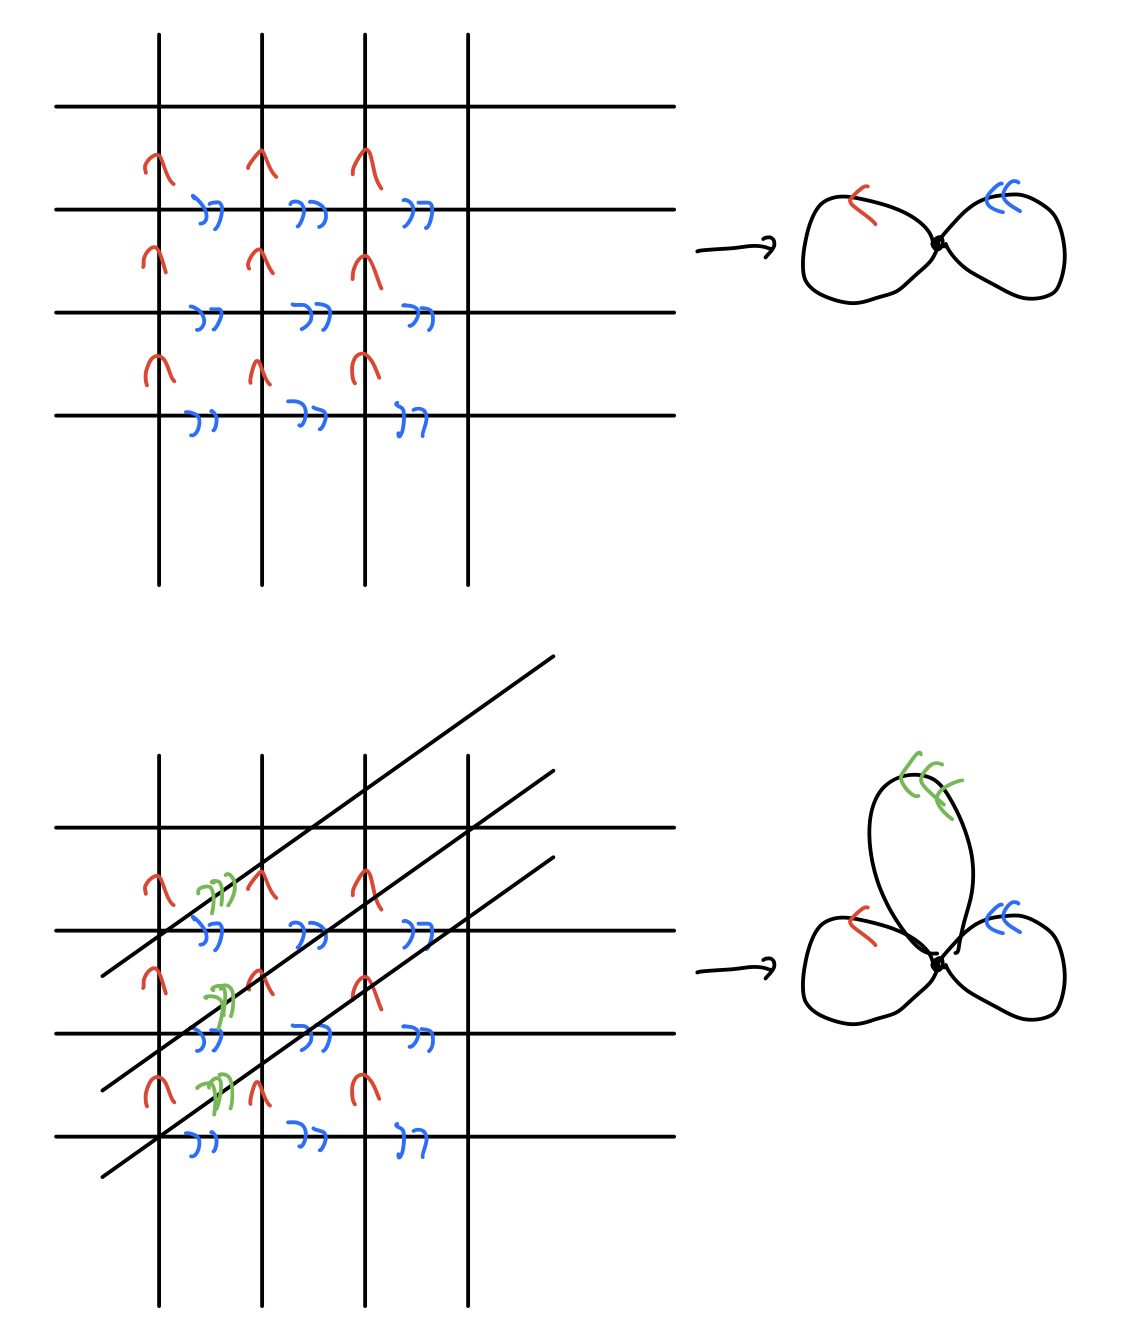
\includegraphics[width=.5\linewidth]{problem18_s1_s1.jpeg}
    \caption{Universal abelian coverings of $S^1 \vee S^1$ and $S^1 \vee S^1 \vee S^1$}
    \label{fig:problem18_s1_s1}
  \end{figure}
\end{proof}

\begin{lem}
  Let $G$ be a group and $H$ be a subgroup.
  If $[a, b] \in H$ for all $a, b \in G$, then $H$ is a normal subgroup of $G$.
\end{lem}

\begin{proof}
  Let $g \in G, h \in H$.
  Then $ghg^{-1} = ghg^{-1}h^{-1}h = [g, h]h$.
  Since $[g, h] \in H$ and $h \in H$, $ghg^{-1} = [g, h]h \in H$.
  Thus $H$ is normal.
\end{proof}

\begin{exer}{(Problem 19)}
  Use the preceding problem to show that a closed orientable surface $M_g$ of genus $g$ has a connected normal covering space with deck transformation group isomorphic to $\mathbb{Z}^n$ (the product of $N$ copies of $\mathbb{Z}$) if and only if $n \leq 2g$.
  For $n = 3$ and $g \geq 3$, describe such a covering space explicitly as a subspace of $\mathbb{R}^3$ with translations of $\mathbb{R}^3$ as deck transformations.
\end{exer}

\begin{proof}
  Suppose $n \leq 2g$.
  Then $\pi_1(M_g) = \ev{a_1, \cdots, a_{2g} \mid [a_1, a_2] \cdots [a_{2g - 1}, a_{2g}]}$.
  Let $H$ be the subgroup of $\pi_1(M_g)$ generated by $a_{n + 1}, \cdots, a_{2g}$ and the set $\{ [a_i, a_j] \mid i \ne j \}$.
  Since $H$ is a subgroup of $\pi_1(M_g)$, there exists a covering space $p: \tilde{M_g} \rightarrow M_g$ by Theorem 1.38 such that $p_*(\pi_1(\tilde{M_g})) = H$.

  By Lemma 0.1 above, $H$ is normal, so, by Proposition 1.39(a), $\tilde{M_g}$ is normal.

  By Proposition 1.39(b), $G(\tilde{M_g})$ is isomorphic to the quotient $N(H) / H$.
  Since $H$ is normal, $N(H) = \pi_1(M_g)$.
  Therefore, $G(\tilde{M_g})$ is isomorphic to $\pi_1(M_g) / H$ where $H$ contains all commutators of $\pi_1(M_g)$.
  Thus $G(\tilde{M_g})$ is abelian, so $\tilde{M_g}$ is an abelian covering space.

  Moreover,
  \begin{align*}
    G(\tilde{M_g})
      &= \pi_1(M_g) / H \\
      &= \ev{a_1, \cdots, a_{2g} \mid a_{n + 1}, \cdots, a_{2g}, \forall i, j, [a_i, a_j]} \\
      &= \ev{a_{1}, \cdots, a_{n} \mid \forall i, j, [a_i, a_j]} \\
      &= \ev{a_{1}, \cdots, a_{n} \mid \forall 1 \leq i < j \leq n, [a_i, a_j]} \\
      &\cong \mathbb{Z}^n.
  \end{align*}
  On the other hand, let $n \in \mathbb{N}$ be given and suppose that there exists a connected normal covering space $\tilde{M}_g$ with deck transformation group isomorphic to $\mathbb{Z}^n$.
  Let $H = p_*\pi_1(\tilde{M}_g)$.
  Then $\mathbb{Z}^n \cong G(\tilde{M}_g) = N(H) / H$.
  Since the deck transformation group is normal and abelian, $H$ is normal and $[\pi_1(M_g), \pi_1(M_g)] \leq H$ by \eqref{eq:abelian} from Problem 18.  

\end{proof}

\begin{exer}{(Problem 20)}
  Construct non-normal covering spaces of the Klein bottle by a Klein bottle and by a torus.
\end{exer}

\begin{proof}
  Figure \ref{fig:non_normal_covering_klein} is the idea that I have for the first part.
  But I don't know how to show that there exists no deck transformation with that permutation.
  \begin{figure}
    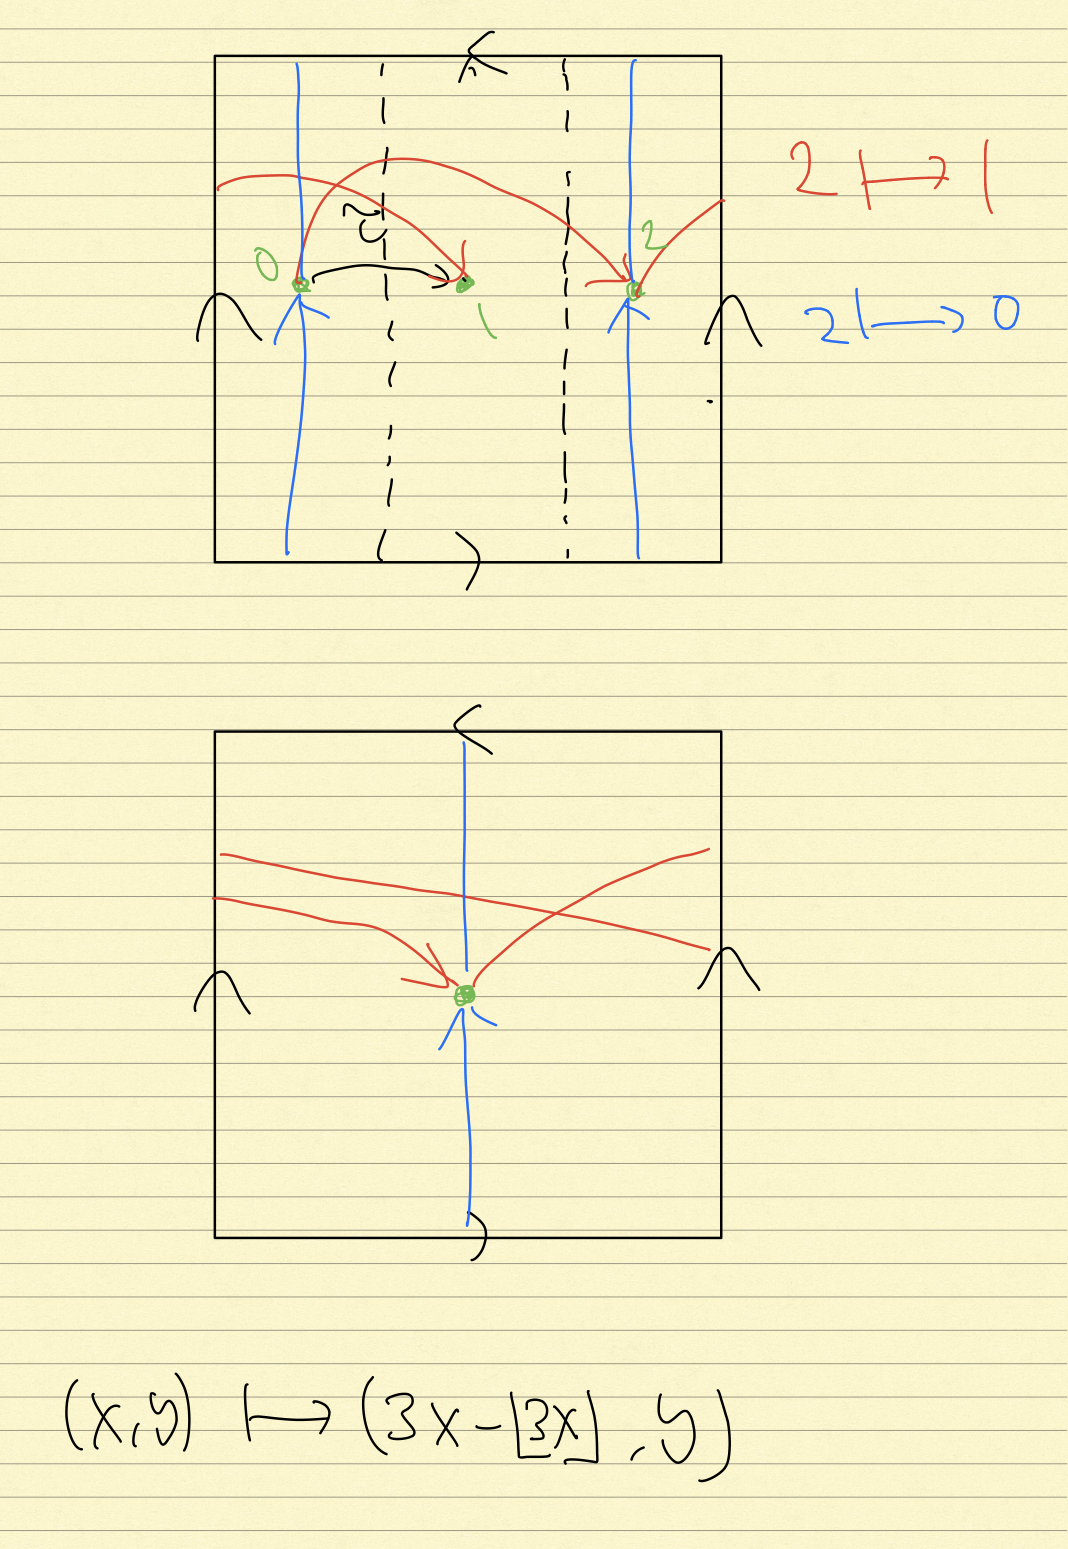
\includegraphics[width=.5\linewidth]{non_normal_covering_klein.jpeg}
    \caption{Problem 20 (Klein)}
    \label{fig:non_normal_covering_klein}
  \end{figure}

  \begin{figure}
    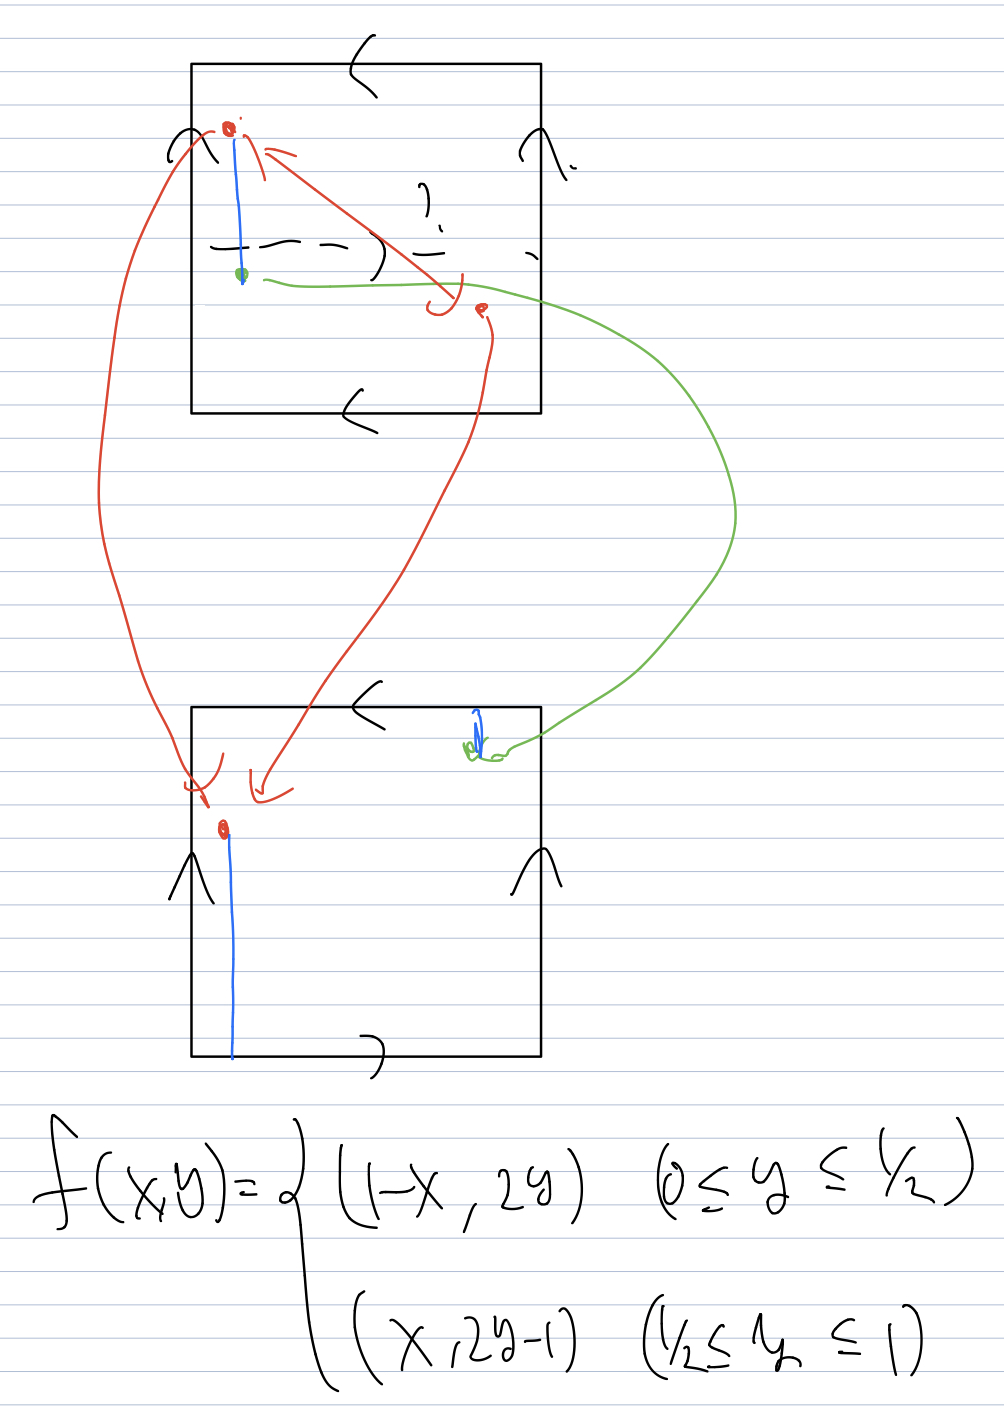
\includegraphics[width=.5\linewidth]{non_normal_covering_torus.jpeg}
    \caption{Problem 20 (Torus)}
    \label{fig:non_normal_covering_torus}
  \end{figure}
  
\end{proof}

\end{document}


